
% \chapter{High Level Architecture - SysML}


The "Management of Modes and Levels" function is mainly described in chapter 4 and 5 of \citep{subset-026}. Modes and levels define the status of the ETCS in regards of on-board functional status and track infrastructure.

\begin{landscape}
\begin{figure}[hbtp]
\centering
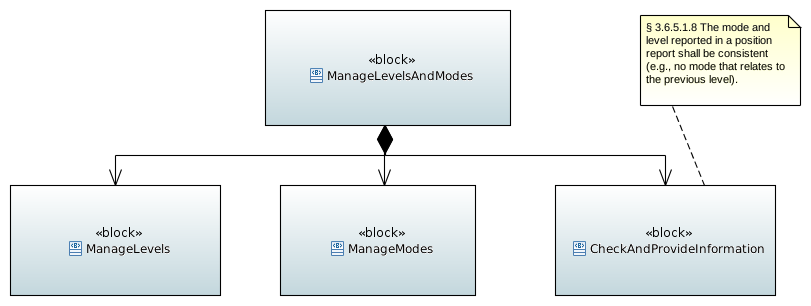
\includegraphics[scale=1]{../SysML/FunctionalArchitecture.png}
\caption{High level Architecture}
\end{figure}
\end{landscape}

This function is shared in three subfunctions: 
\begin{description}
\item[Manage modes] computes the new mode to apply according conditions from inputs and other functions (see \citep{subset-026} sections 4.4, 4.6, 5.4, 5.5, 5.6, 5.7, 5.8, 5.9, 5.11, 5.12, 5.13, 5.19)
\item[Manage levels] computes the new level to apply according inputs (see \citep{subset-026} section 5.10)
\item[Provide output] checks compatibility between mode and level and provides outputs (see \citep{subset-026} section 3.6.5)
\end{description}

\begin{landscape}
\begin{figure}[hbtp]
\centering
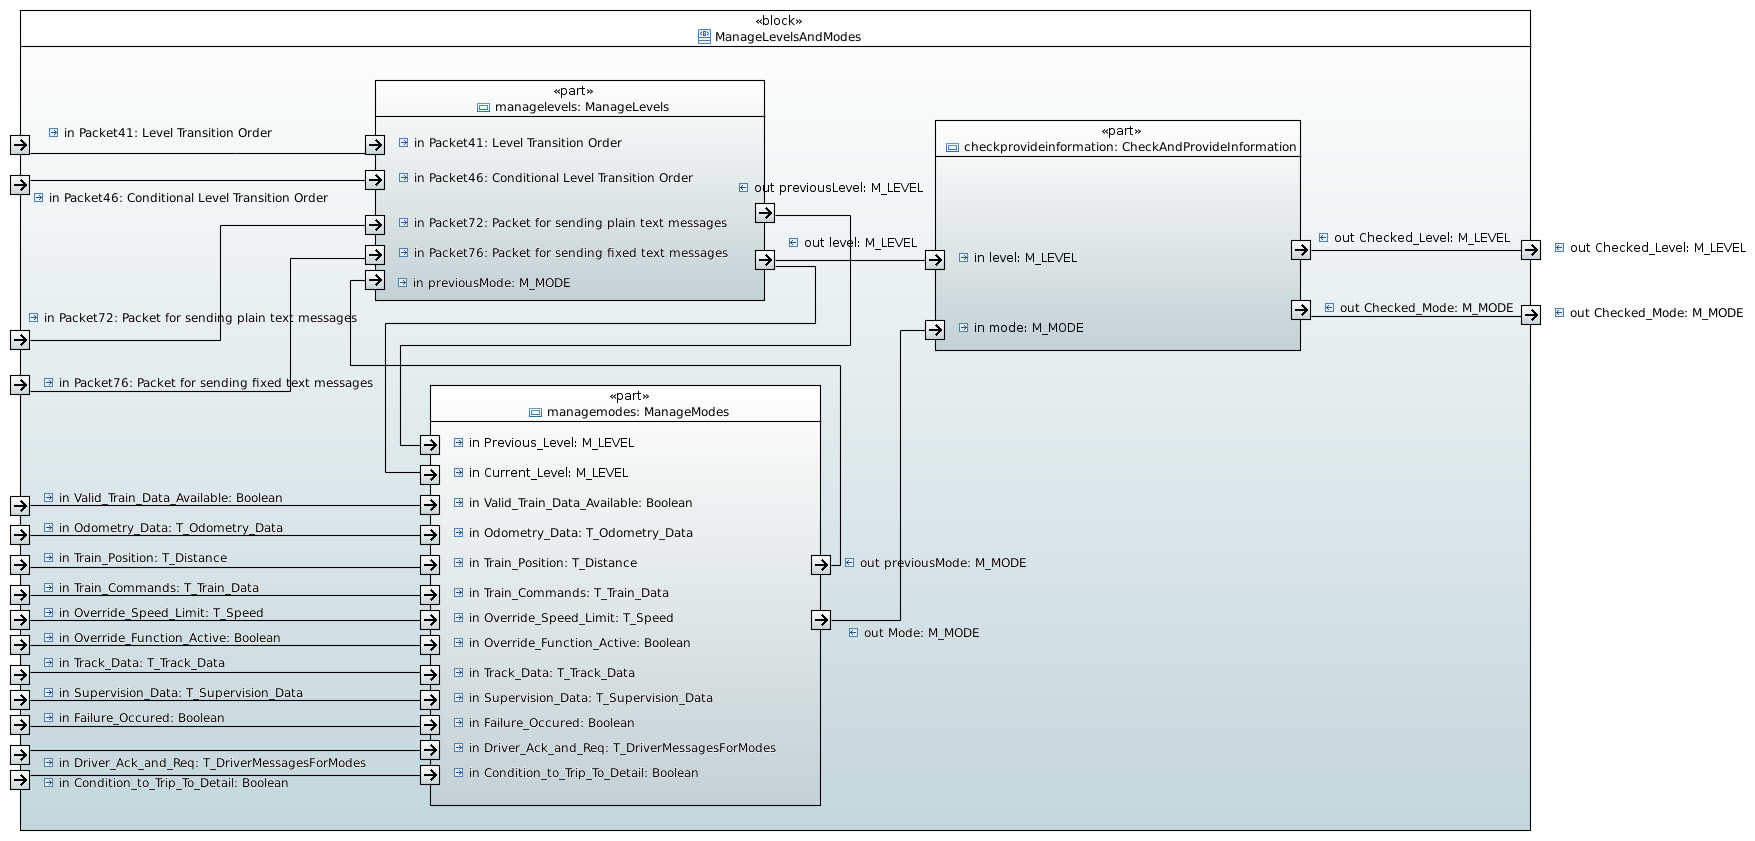
\includegraphics[scale=0.6]{../SysML/ManageLevelsAndModes.png}
\caption{High level dataFlow}
\end{figure}
\end{landscape}

The previous figure show the main interface of this function, according to the type defined as follow:

\begin{landscape}
\begin{figure}[hbtp]
\centering
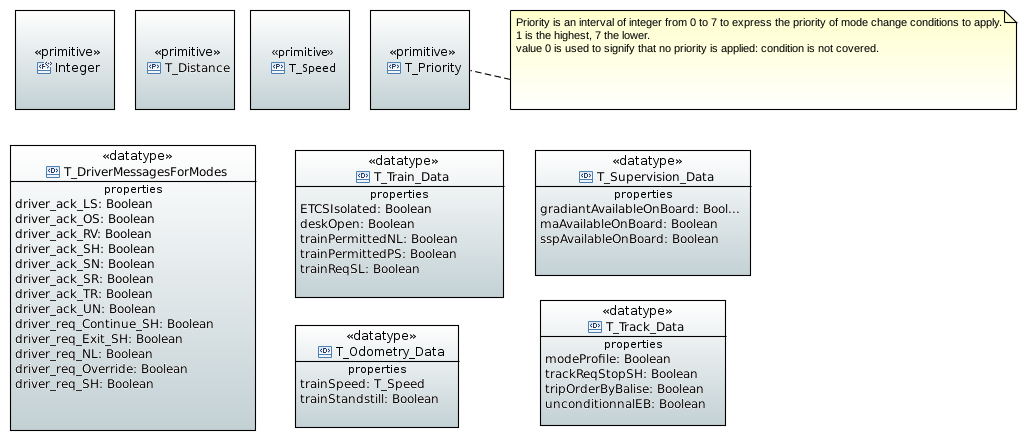
\includegraphics[scale=0.9]{../SysML/DataTypes.png}
\caption{Data Types}
\end{figure}
\end{landscape}

% end of chapter